\chapter{Testing, Results and Critical Analysis}
\minitoc
\newpage

\setcounter{secnumdepth}{0}
\section{Introduction}
This chapter validates the implementation described in the 
previous chapter by presenting the results obtained at each 
stage of the project. It then concludes with a critical 
analysis of what was achieved, the limitations encountered, 
and the improvements that could be made in the future.

\setcounter{secnumdepth}{2}

% ----------------------- Infrastructure Validation ----------------------- %
\section{Infrastructure Validation}
This section verifies that the AWS infrastructure provisioned 
by Terraform was created correctly and that the cluster is 
healthy and ready to receive workloads.



% ----------------------- Application Deployment Validation ----------------------- %
\section{Application Deployment Validation}
This section verifies that the three Mashroom applications 
are correctly deployed and running on the EKS cluster, 
confirming that the Kubernetes configuration and ArgoCD 
setup are functioning as expected in the cloud environment.

\subsection{ArgoCD Sync Status}
Figure \ref{fig:argocd-dashboard} shows the ArgoCD dashboard 
with all three applications in a healthy and synced state. 
The root application successfully deployed both the 
\texttt{prod} and \texttt{staging} environments, each 
pointing to their corresponding Kustomize overlay in 
the GitOps repository.

\begin{figure}[H]
    \centering
    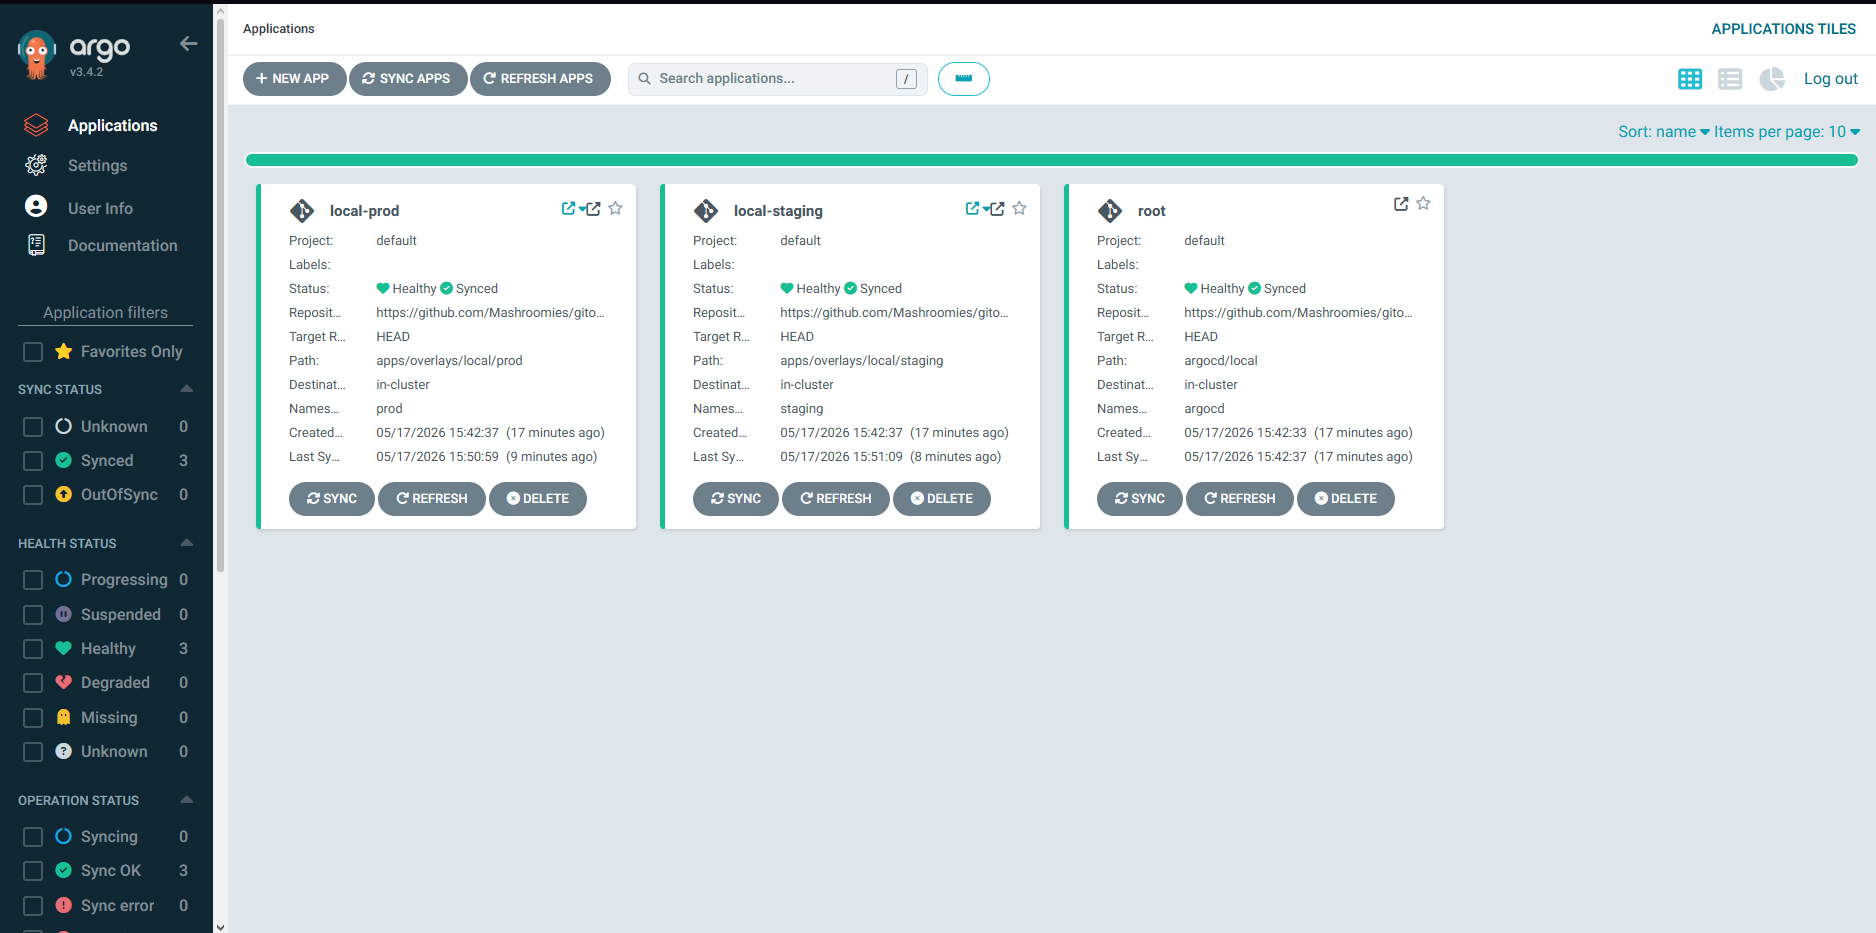
\includegraphics[width=0.9\linewidth]{src/assets/images/argocd-dashboard.png}
    \caption{ArgoCD dashboard showing all applications healthy and synced}
    \label{fig:argocd-dashboard}
\end{figure}

\subsection{Running Pods and Services}
Figure \ref{fig:pods-running} shows the ArgoCD resource tree 
for the production environment. Incoming traffic enters through 
the Ingress, gets routed to each application's Service, and 
reaches the corresponding running pod. All three applications, 
the API, the Landing Page, and the Studio, are in a healthy 
and running state.

\begin{figure}[H]
    \centering
    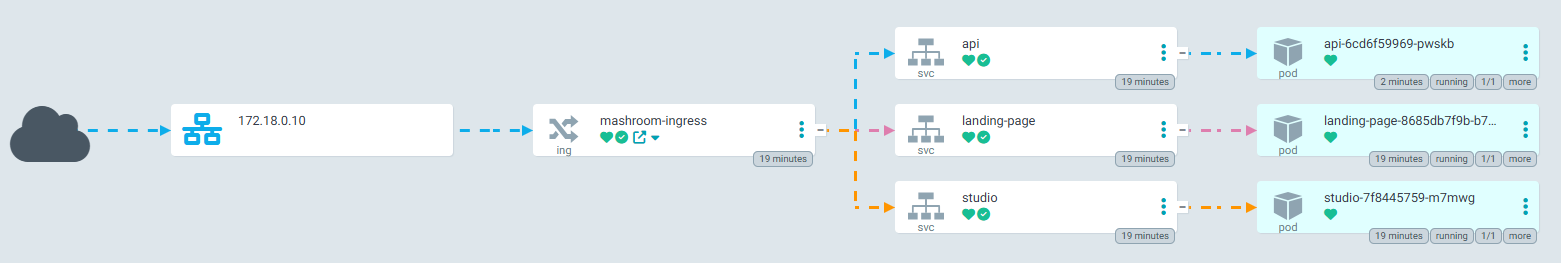
\includegraphics[width=1\linewidth]{src/assets/images/pods-running.png}
    \caption{ArgoCD resource tree showing all pods running and healthy}
    \label{fig:pods-running}
\end{figure}

\subsection{Application Accessibility}
.....

% ----------------------- CI/CD Pipeline Validation ----------------------- %
\section{CI/CD Pipeline Validation}
This section verifies that the CI/CD pipelines are functioning 
correctly, from the GitHub Actions workflow runs to the 
automatic update of the GitOps repository that triggers 
the deployment.

\subsection{GitHub Actions Workflow Results}
Figure \ref{fig:gh-actions-results} shows a successful pipeline 
run triggered by a push to \texttt{main}. The build job 
completed in 40 seconds and the GitOps update job ran 
immediately after, confirming that the image tag was 
automatically updated in the GitOps repository.

\begin{figure}[H]
    \centering
    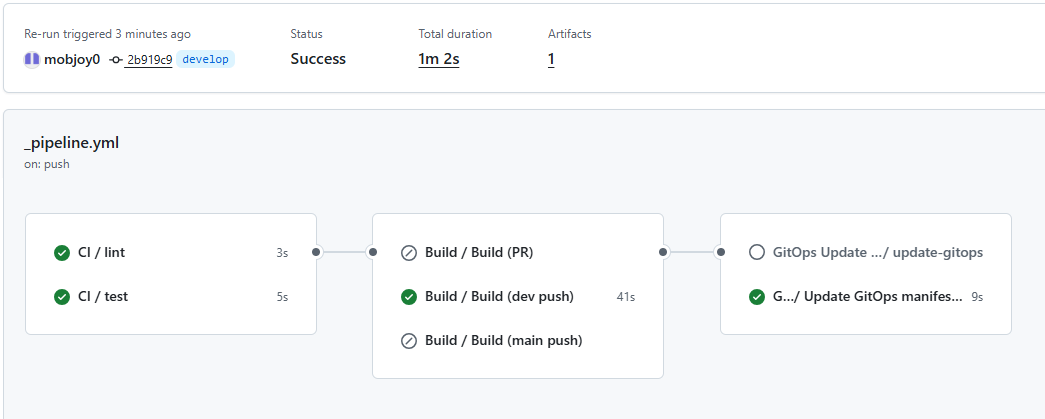
\includegraphics[width=0.9\linewidth]{src/assets/images/gh-actions-results.png}
    \caption{Successful GitHub Actions pipeline run}
    \label{fig:gh-actions-results}
\end{figure}

\subsection{Automated Synchronization}
This subsection checks the final step: that ArgoCD applies 
the GitOps change to the cluster on its own.

After the workflow committed the new image tag, ArgoCD saw 
that the cluster no longer matched the repository. With the 
automated sync policy enabled, it updated the cluster to the 
new version with no manual action, as shown in figure 
\ref{fig:argocd-autosync}.

\begin{figure}[H]
    \centering
    
\includegraphics[width=0.9\linewidth]{src/assets/images/placeHolder.png}
    \caption{ArgoCD syncing the cluster automatically after a GitOps commit}
    \label{fig:argocd-autosync}
\end{figure}

This confirms the full loop: a merge into \texttt{main} builds 
the image, updates the tag, and ArgoCD syncs the cluster, with 
no manual steps from commit to deployment.

% ----------------------- Critical Analysis ----------------------- %
\section{Critical Analysis}
This section reflects on the work carried out throughout 
the internship, evaluating what was achieved against the 
objectives defined in chapter 1, acknowledging the limitations 
encountered, and identifying areas that could be improved 
in future iterations of the project.

\subsection{Achieved Objectives}
The new architecture was designed to address the six weaknesses 
identified in section 1.3.1. This subsection revisits each one and 
shows how the new system resolves it.

\subsubsection{Eliminating the Single Point of Failure}
The platform no longer runs on a single machine. The EKS cluster 
spans multiple nodes, and each application runs as several 
replicas spread across them. If a node or a pod fails, Kubernetes 
reschedules the workload automatically, with no manual action.

\subsubsection{Scalability}
To measure the improvement, a stress test was run against the 
old VM setup and the new cluster under the same load.

Figure \ref{fig:stress-test} compares the two. The old VM 
started failing requests at X concurrent users, while the cluster 
scaled horizontally and kept serving traffic up to Y users without 
errors.

\begin{figure}[H]
    \centering
    
\includegraphics[width=0.9\linewidth]{src/assets/images/placeHolder.png}
    \caption{Stress test results comparing the old VM and the new cluster}
    \label{fig:stress-test}
\end{figure}

\subsubsection{Automated Deployments}
Releases are no longer performed by hand on the server. As shown 
in sections 4.3.1 and 4.3.2, a merge into \texttt{main} now triggers 
the full pipeline from image build to cluster sync, with no manual 
steps.
\subsubsection{Environment Separation}
The cluster runs two isolated environments, \texttt{staging} and 
\texttt{prod}, each in its own namespace and managed by its own 
Kustomize overlay. Changes can now be tested in staging before 
reaching real users.

\subsubsection{Reproducible Infrastructure}
The entire infrastructure is defined as Terraform code stored in 
Git. The same setup can be destroyed and rebuilt from scratch with 
a single \texttt{terraform apply}, removing the manual server 
configuration that the old setup relied on.

\subsubsection{Lower Operational Cost}
Manual deployments previously required a developer to connect 
to the server, pull the latest code, install dependencies, and 
restart the service, a process that could take up to 15 minutes 
and was prone to human error. The CI pipeline now completes the 
build and push in under 40 seconds, as shown in figure 
\ref{fig:gh-actions-results}, and the CD side is fully handled by 
ArgoCD with no manual steps involved.

\subsection{Limitations and Future Improvements}
.....

% ----------------------- Conclusion ----------------------- %
\setcounter{secnumdepth}{0}
\section{Conclusion}